\documentclass[12pt, a4paper, hidelinks]{article}

% Packages:
\usepackage{graphicx}                   % For figure includes
\usepackage[T1]{fontenc}                % For mixing up \textsc{} with \textbf{}
\usepackage[utf8]{inputenc}             % For scandinavian input characters(æøå)
\usepackage{amsfonts, amsmath, amssymb} % For common mathsymbols and fonts
\usepackage[english]{babel}              % For danish titles
\usepackage{hyperref}                   % For making links and refrences
\usepackage{url}                        % Just because {~_^}
\usepackage{array}                      % ...
\usepackage[usenames, dvipsnames, svgnames, table]{xcolor}
\usepackage{tabularx, colortbl}
\usepackage{verbatim} % For entering code snippets.
\usepackage{fancyvrb} % A "fancy" verbatim (for pseudo code).
\usepackage{listings} % For boxed codesnippets, and file includes. (begin)
\usepackage{lipsum}   % For generating dummy text at this demonstration
\usepackage{enumitem}
\usepackage[section]{placeins} % prevents figures from floating
\usepackage[final]{pdfpages}   % for including the frontpage
\usepackage{makecell}          % for heavier \hlines
\usepackage{caption}           % for costum captions
\usepackage{cleveref}          % for cref

% Basic layout:
\setlength{\textwidth}{165mm}
\setlength{\textheight}{240mm}
\setlength{\parindent}{0mm}
\setlength{\parskip}{\parsep}
\setlength{\headheight}{0mm}
\setlength{\headsep}{0mm}
\setlength{\hoffset}{-2.5mm}
\setlength{\voffset}{0mm}
\setlength{\footskip}{15mm}
\setlength{\oddsidemargin}{0mm}
\setlength{\topmargin}{0mm}
\setlength{\evensidemargin}{0mm}

\newcolumntype{C}[1]{>{\centering\arraybackslash}p{#1}}

% Colors:
\definecolor{KU-red}{RGB}{144, 26, 30}

% Text Coloring:
\newcommand{\green}[1]{\textbf{\color{green}{#1}}}
\newcommand{\blue} [1]{\textbf{\color{blue} {#1}}}
\newcommand{\red}  [1]{\textbf{\color{red}  {#1}}}
% Create a figure with \fig{filename}{figure_text}
\newcommand{\fig}[3]{
\begin{figure}[h]
  \begin{center}
    \includegraphics[width=#2mm]{./img/#1}
  \end{center}
  \caption{#3}
  \label{fig:#1}
\end{figure}
}
\def\fatline{\Xhline{2\arrayrulewidth}}
\renewcommand{\arraystretch}{1.3}
\renewcommand{\tt}[1]{\texttt{#1}}
\renewcommand{\bf}[1]{\textbf{#1}}
\renewcommand{\it}[1]{\textit{#1}}

% **************** Start Document *****************
\begin{document}
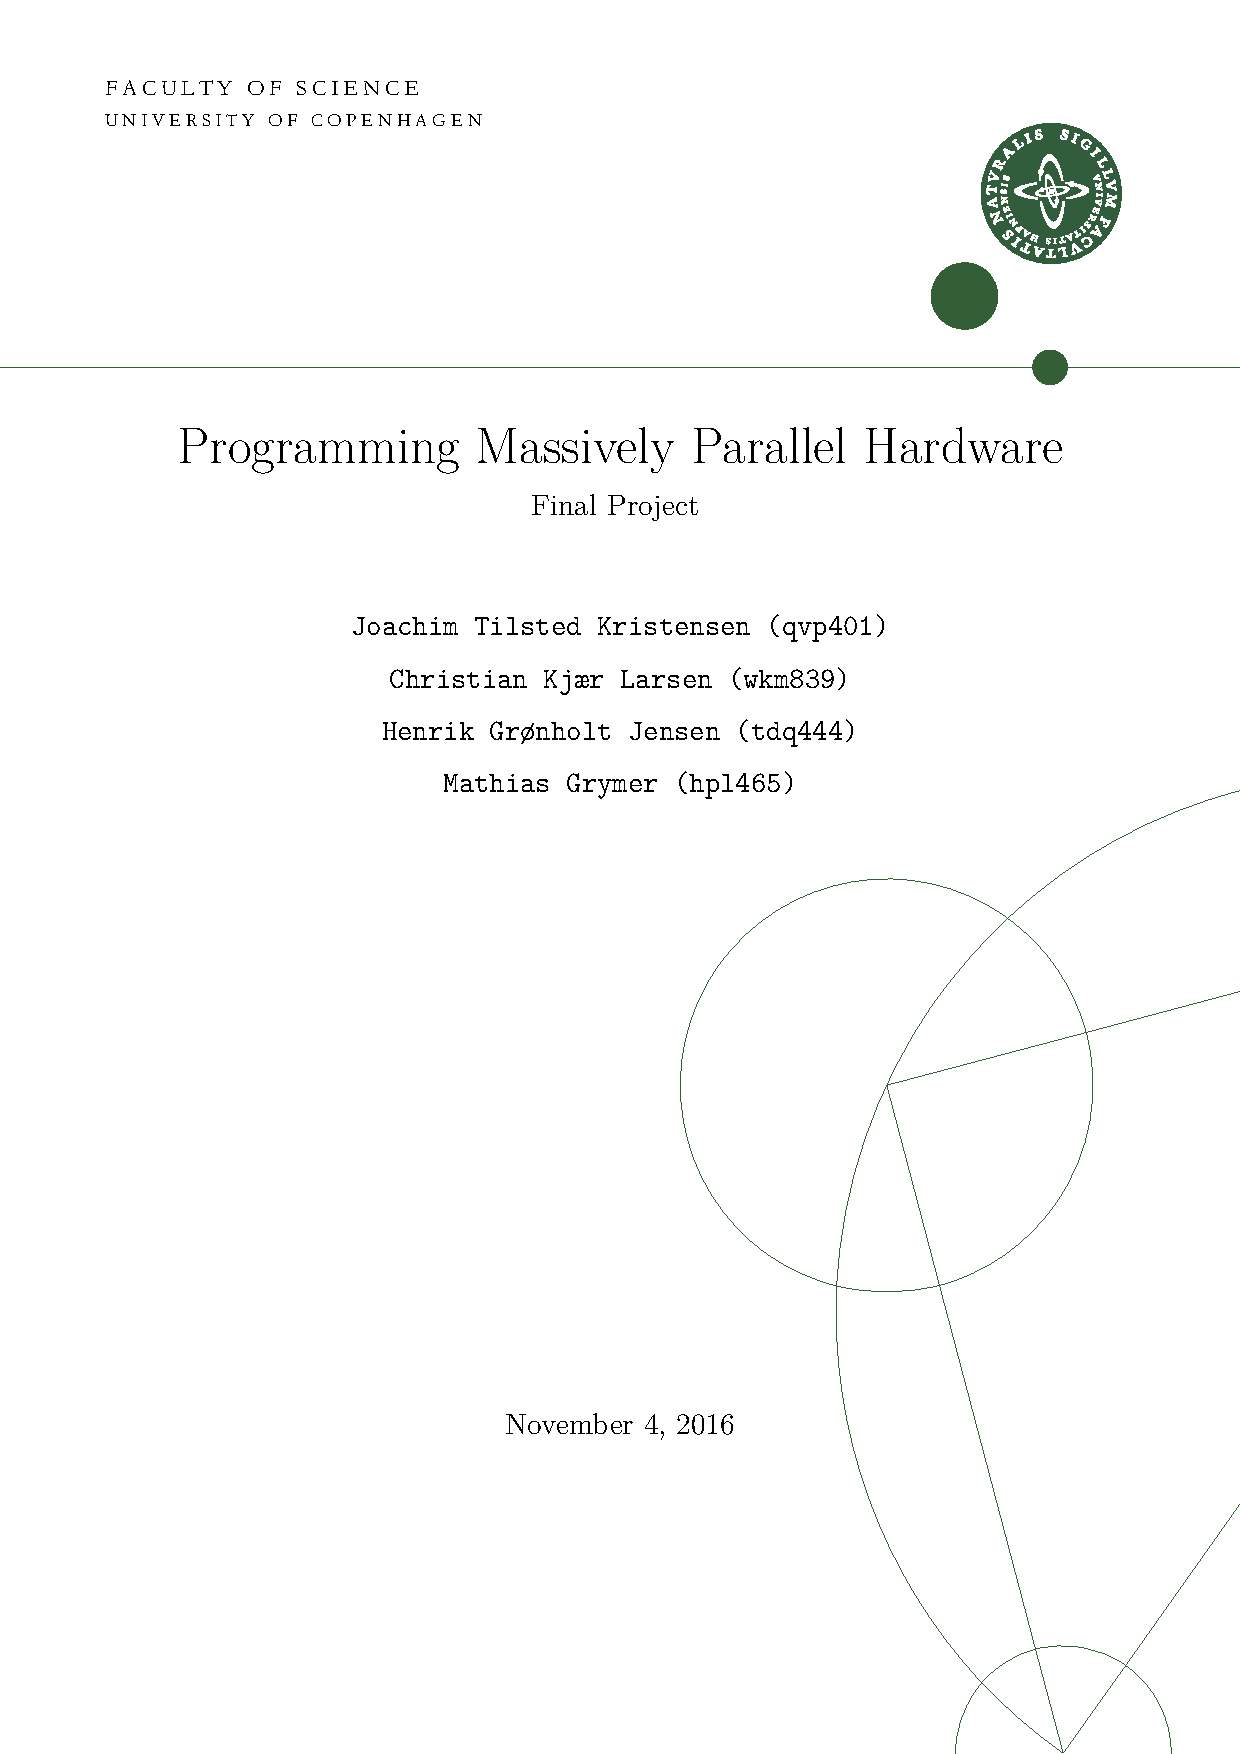
\includepdf[pages=1]{./frontpage/frontpage.pdf}
\tableofcontents
\newpage

\section{Project Introduction}
A histogram is a density estimate over a distribution of data.
It is quintessential to quality control, distribution estimation
and similarity measures when working with large datasets.
As the time it takes to compute the histogram scales with the size of the input,
a parallel solution is preferable when the input is large.
However, when it comes to real world unsorted data,
histograms are computationally inefficient
due to the random memory access pattern related to counting of how many values fall into each bin.
In this project, we implement a CUDA-based solution for building a 1D histogram
in parallel and benchmark the scalability of our solution with
the CPU and a naive GPU version.
We also investigate how to efficiently solve the problem when the dataset
is larger than the available (device) memory on the GPU
using streaming techniques.

\section{Design Overview - From CPU to GPU}
Building a histogram in parallel is a straightforward map-reduce problem.
It can be thought of as simplistic kernel density estimation,
where a function $f$ maps frequencies of \tt{data} over bins \tt{inds}
and reduces by counting how many values falls into each bin.
Hence, pseudo-code for a 1D histogram would look something lke:

\begin{verbatim}
forall (i = 0; i < size(data); i++)
    inds = f(data[i])
    hist[idx]++ // Must be atomic
\end{verbatim}

Unfortunately, writing an efficient parallel implementation
yields a number of problems related to memory performance.
One of these is the unknown order of indices from the map-phase which
prevents us from working with the data in a coalesced
manner during the reduce-phase.

\subsection{Optimising for Memory Performance}
Since the \tt{inds} array is unpredictable,
we expect worse cache performance with an increasing number of bins.
As the number of bins increase the range of possible
memory addresses increase as well. At some point we reach a size where
we often have to bring in data from global memory instead of working
from cache.

Since random accesses to global memory on the GPU are very
expensive, and result in a lot of cache misses, we would like
to work on parts of the histogram where all memory accesses
can fit into the fast shared memory for each CUDA block.

This means that the cuda kernel has to work on small local histograms
which fit into shared memory, and flush back into corresponding parts of the global histogram.

In practice, this means partially sorting the
input data into \it{segments} where values in a particular \it{segment}
all contribute to the same small \tt{gpu\_hist\_size} number of bins.

Since the \tt{gpu\_hist\_size} is a fixed number
decided by the number of bins which can be held in the shared device memory,
and since the segment that a particular index value falls into
is (\tt{index\_value / gpu\_hist\_size}),
we decided to partially sort the indices by bits that are more significant than those
lower than \tt{gpu\_hist\_size} using radix sort. Radix sort has an efficient GPU
implementation in the Cub library for the CUDA API\footnote{\url{https://nvlabs.github.io/cub/}}.


\subsection{A Memory Effecient Algorithm}
%% Theoretically, the amount of time needed to compute a histogram is
%% proportional with the greatest number of additions to a single bin.
%% In practice however, this is not the case:\\
As the available parallelism is limited by the physical device resources,
an ideal algorithm is essentially one that fully utilizes the hardware.
For us this means dividing the workload into
equally sized \it{chunks}, such that the size of a \it{chunk} is
\tt{total\_workload / hardware\_parallelism},
where the total workload is the size of the data input,
and the available hardware parallelism is the total number of threads available.

This is achived by having each CUDA block create a local histogram in shared memory
which is atomically added to a global histogram residing on the GPU.
It is very likely that some blocks working on such large subsets of data will
be working on more than one \it{segment}.

So, in each CUDA block we need to know when to flush a local histogram to global
memory and start working on another one.
The subset of values that a block handles is defined as the \tt{chunk\_size}
multiplied by the number of threads in a block (\tt{\#thread\_pr\_block}).
A high level example of such an algorithm is illustrated in \Cref{fig:overview}
where e.g. $block_0$ spans $segment_0$ and $segment_1$.

\fig{overview}{140}{General idea of the algorithm}

Letting a block handle overlapping segments (i.e. creating more local histograms)
is preferable to a more naïve implementation where a block is spawned
for each segment. This is because there is no way to guarantee that all blocks have
roughly the same workload.
One could easily have a case where certain segments have significantly
more elements than others, leading to bottlenecks where other blocks will
wait for the overworked blocks to finish.

\section{Overview of Implementation}
In this section, we give a quick overview of our implementation.
First we describe an implementation with shared memory which does not handle
histograms larger than what fits in shared memory on the GPU.
Then we describe an implementation for histograms of arbitrary size,
which introduces some extra bookkeeping to make everything work.

\fig{device-dia}{140}{Flow of data in our GPU implementation}

\subsection{Optimised for small histograms}
The first step towards the algorithm described previously is an implementation
for histograms less than the size of the shared memory available for a CUDA block.
Since this around 8000 words of memory,
we used a \tt{gpu\_hist\_size} of 4096/8192 elements (depending on the configuration).
The reason for using less than the available shared memory, is that the hardware can
reconfigure parts of shared memory to function as a cache, hence speeding
up other memory accesses.

The algorithm is roughly:

\begin{itemize}
\item Reset shared memory.
\item Write the indices (\tt{f(data[i])}) into the block level histogram.
\item Commit the block level histogram to global memory.
\end{itemize}

We also divide the input array into chunks, to avoid having to flush the
local histogram too often. This is done in the way described in the previous section
such that we still exploit all available parallelism.

\subsection{Optimised for large histograms}
For larger histograms, the algorithm needs an expansion in the form
of extra bookkeeping, which depends on a small amount of extra information, and
the input data invariant, that all elements which belongs to the same segment,
are located consecutively in the \tt{inds} array.
The extra information needed, is then a small \tt{segment\_offset} array,
containing the indices into \tt{inds}, at where each new \it{segment} begins.

The optimized algorithm is roughly:

%% Pseudo Code, more like real code, but still pseudo ?
%% \begin{verbatim}
%% 00.  PRELUDE:
%% 01.       Map f onto the data array
%% 02.       Partially sort the resulting indices into segments
%% 03.       Figure out which segment we are currently working
%% 04.  RESET_SHARED_MEMORY:
%% 05.       Reset the shared memory for the CUDA block
%% 06.  HISTOGRAM_KERNEL:
%% 07.       Write the indices modulo the gpu_hist_size into shared memory.
%% 08.       If (we ended a segment):
%% 09.         Commit the block level histogram;
%% 10.         GOTO: RESET_SHARED_MEMORY;
%% 11.       Else:
%% 12.         Unless, all segments have been commited;
%% 13.         GOTO: HISTOGRAM_KERNEL;
%% \end{verbatim}

\begin{enumerate}
\item Map f onto the data array
\item Partially sort the resulting indices into segments
\item Figure out which segment we are currently working on
\item Reset the shared memory for the CUDA block
\item Write the indices modulo the \tt{gpu\_hist\_size} into shared memory.
\item If we ended a segment $\Rightarrow$ commit the block level histogram to global memory,
      and reset shared memory.
\item Until all segments have been commited. repeat from 5.
\end{enumerate}

Since most of the details are very hardware specific,
we suggest reading the CUDA implementation for more details.
However, we have a flowchart of the code that can be found in \Cref{fig:device-dia}.

\section{Benchmarks}
\label{section:bench}
To evaluate our implementation, we have benchmarked it against
a dataset of 10 million randomly generated elements.
We have kept input data size constant,
as our point of interrest is whether our implementation is more
efficient when the number of bins in the histogram increases.
The result can be seen on figure~\ref{fig:graph1}.

\begin{figure}[htpb]
    \centering
    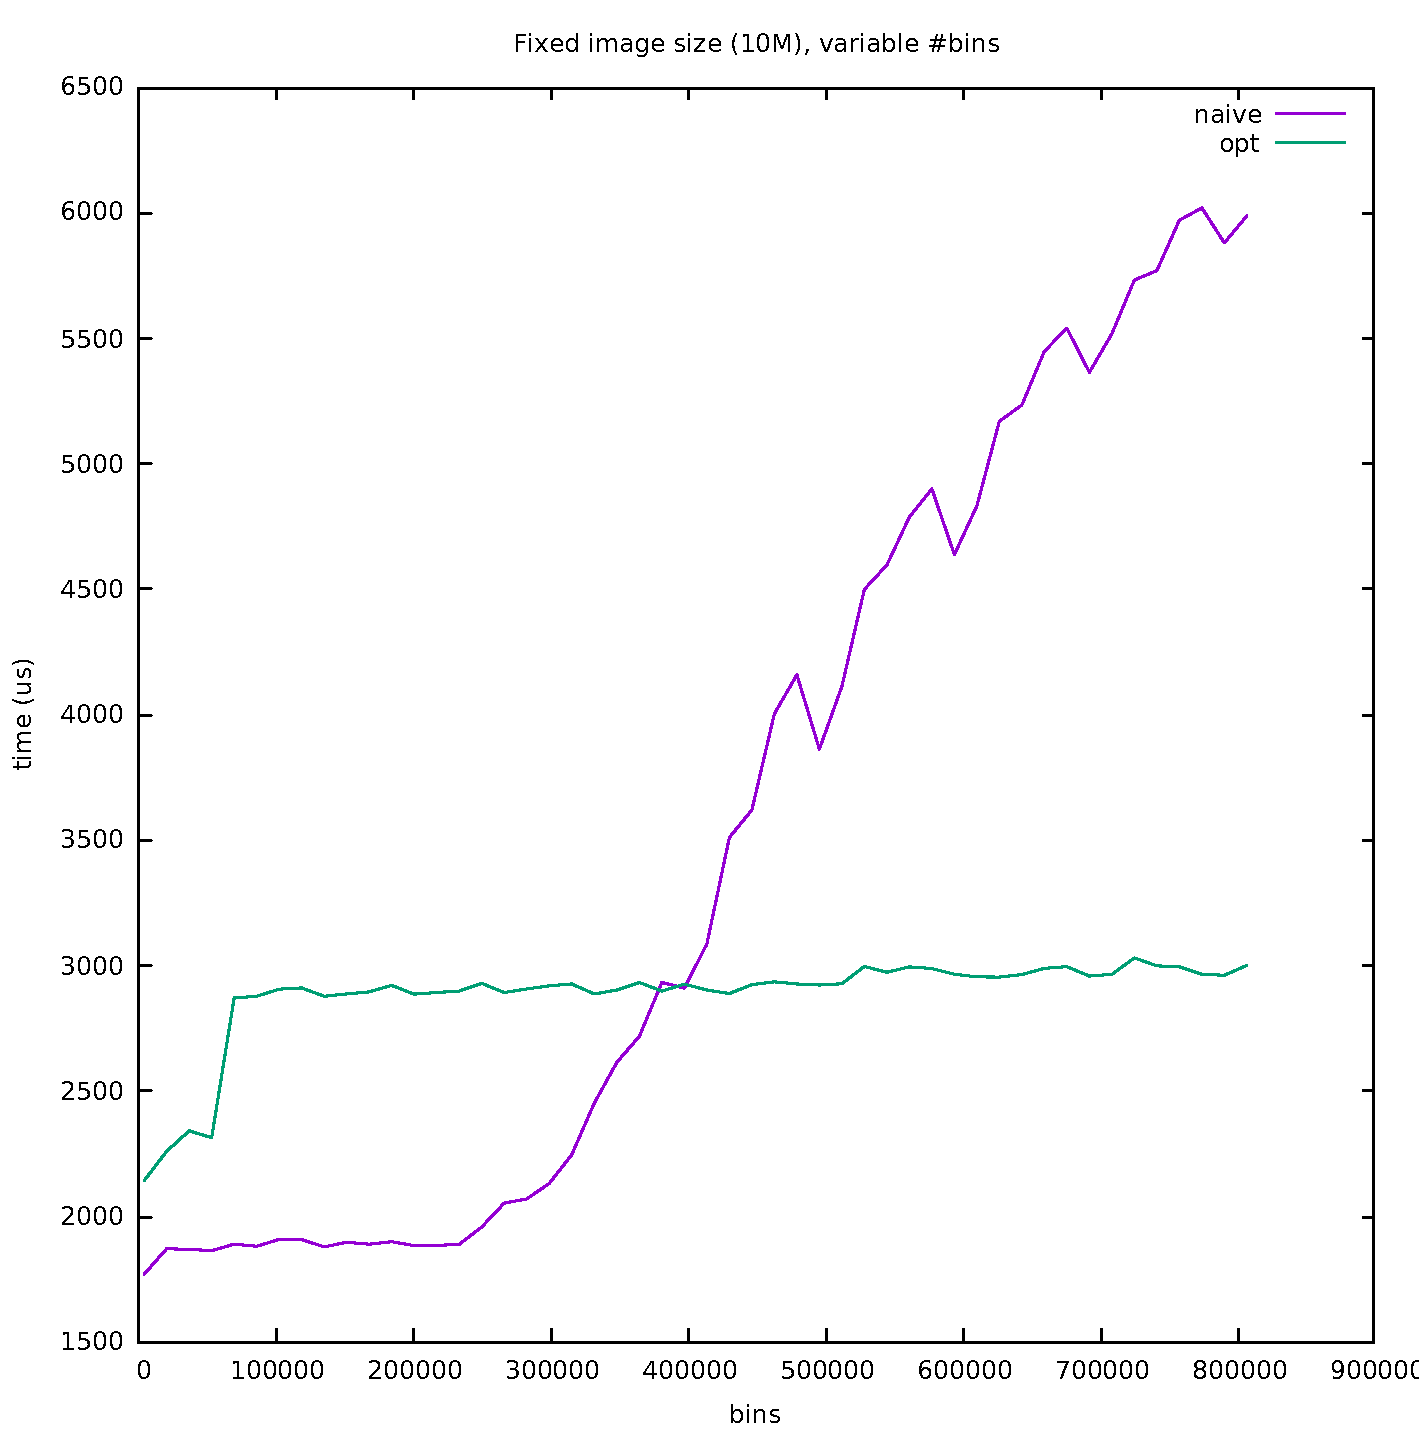
\includegraphics[width=0.6\linewidth]{img/graphs/10M-varbins.pdf}
    \caption{10 million elements with a variable bin count.}
    \label{fig:graph1}
\end{figure}

The benchmark illustrated in \Cref{fig:graph1}
shows that somewhere between 300k and 400k bins
the optimised implementation is faster.
This seems like a lot of bins,
so we used \tt{nvprof} to see what kernels dominated the runtime.
Measurements for 10M elements and 350k bins are shown in \Cref{table:nvprof0}.

\begin{center}
  \begin{tabular}{l|r|r}
    \bf{Kernel} & \bf{Optimised (us)} & \bf{Naive (us)}   \\ \fatline
    \tt{Index and boundary calculation} & $537$  & $537$  \\ \hline
    \tt{Segment offsets}                & $417$  & -      \\ \hline
    \tt{Radix sort}                     & $1228$ & -      \\ \hline
    \tt{Histogram kernel}               & $446$  & $1433$ \\ \fatline
    \bf{Total}                          & $2628$ & $1970$ \\
  \end{tabular}\\
  \captionof{table}{
    The time spent for various kernels,
    at $10^6$ elements and $3.5 \cdot 10^4$ bins.}
  \label{table:nvprof0}
\end{center}

From these results it is clear, that the sorting contibutes as much cost
as the naive histogram kernel.
On a positive note the optimised histogram kernel is about 3 times as
fast as the naive kernel.
A possible explanation might be that radix sort from the Cub library
sorts on more bits than we need.
We also benchmark for a smaller dataset (1M).
This can be seen on figure~\ref{fig:graph2}. The results are similar.

\begin{figure}[htpb]
    \centering
    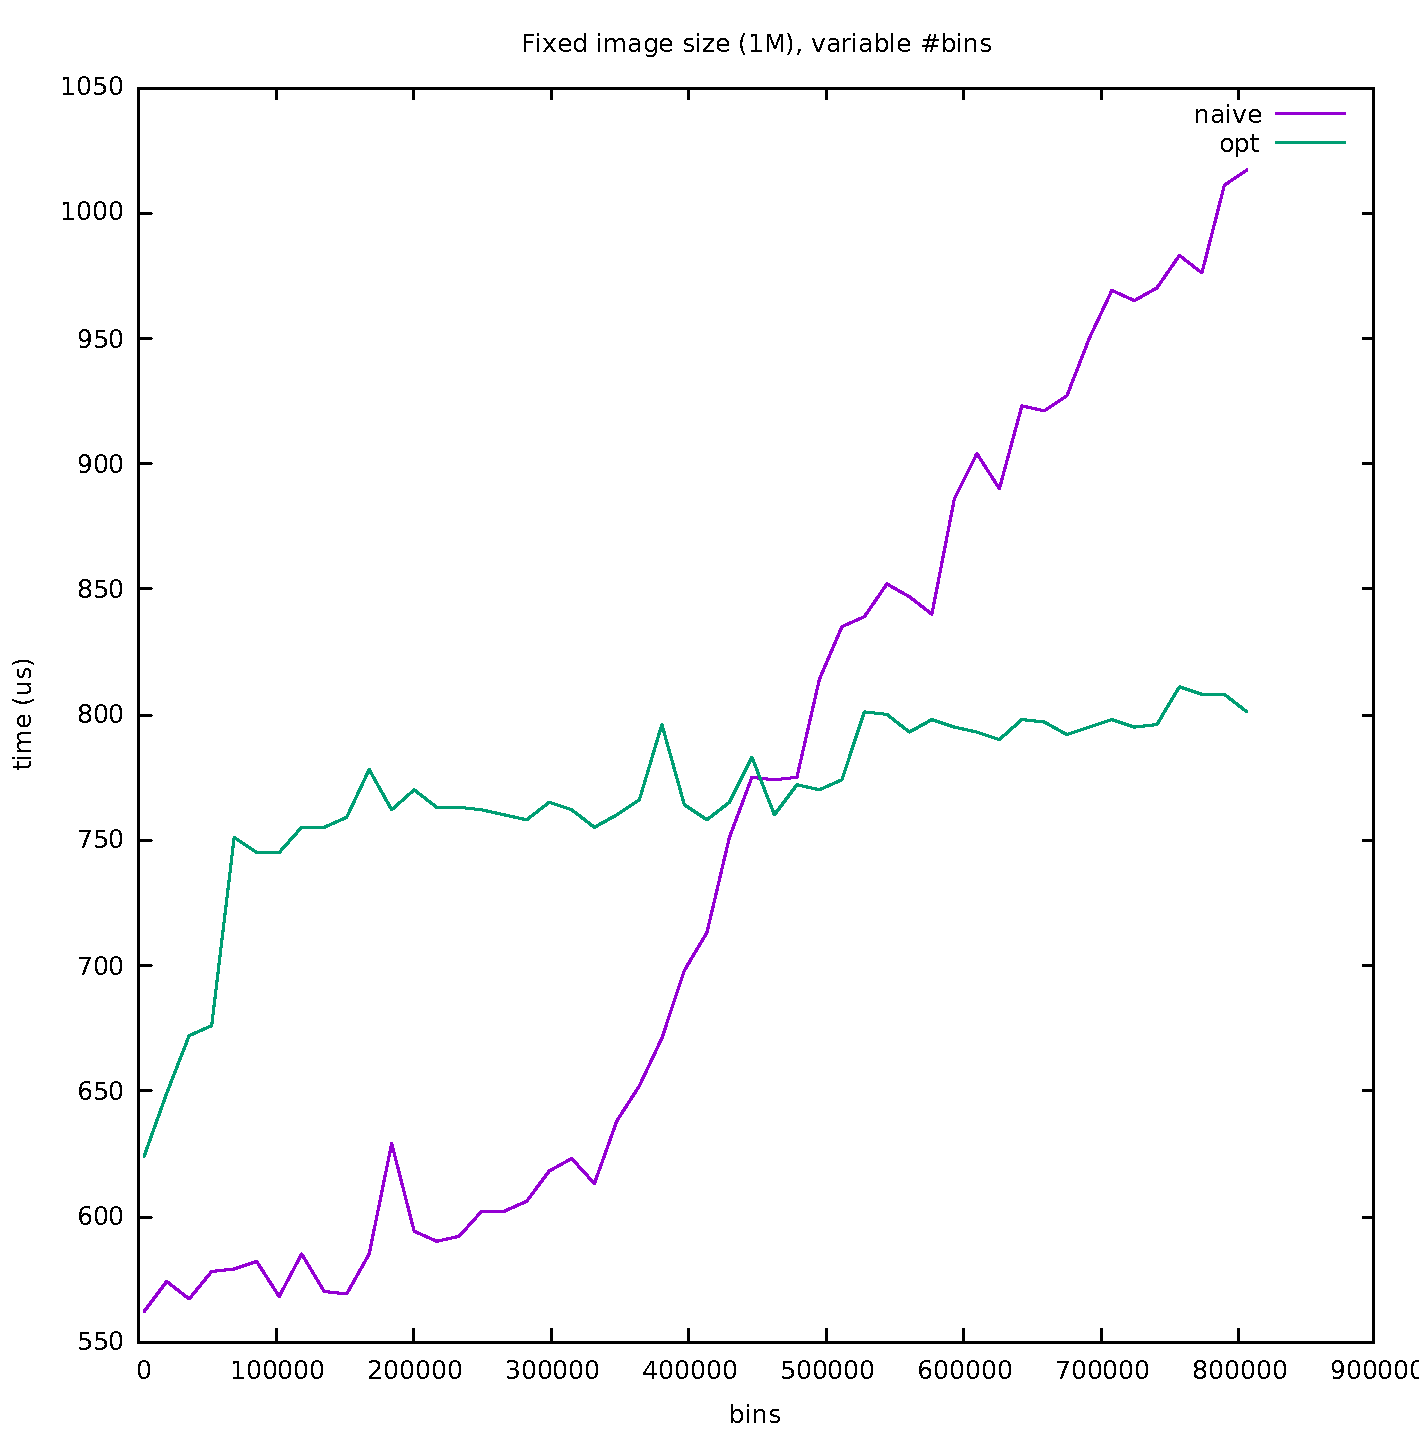
\includegraphics[width=0.6\linewidth]{img/graphs/1M-varbins.pdf}
    \caption{1 million elements with a variable bin count.}
    \label{fig:graph2}
\end{figure}


We have also benchmarked the kernel optimised for smaller histograms. Again we keep the size of the input array constant and vary the number of bins. The result can be seen on figure~\ref{fig:graph3} and on figure~\ref{fig:graph4}. 

\begin{figure}[htpb]
    \centering
    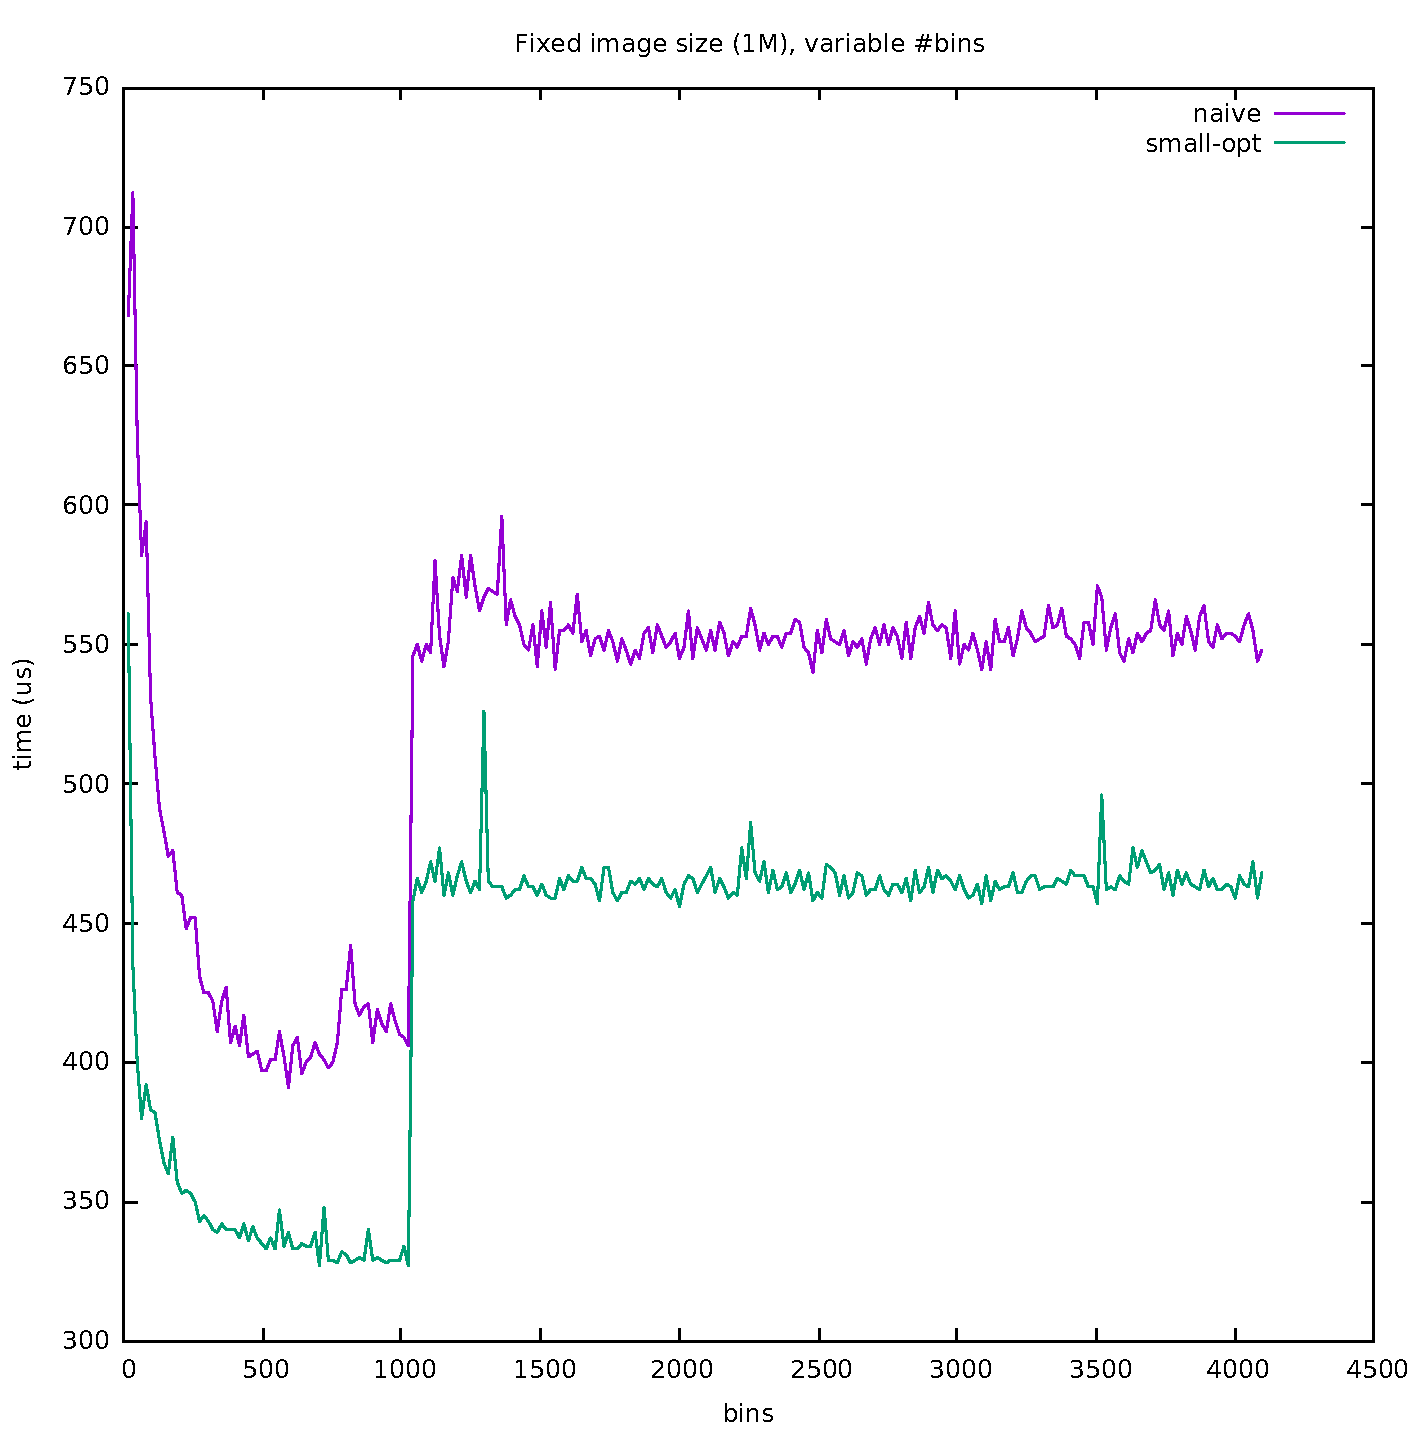
\includegraphics[width=0.6\linewidth]{img/graphs/1M-smallvarbins.pdf}
    \caption{1 million elements with a small variable bin count.}
    \label{fig:graph3}
\end{figure}
\begin{figure}[htpb]
    \centering
    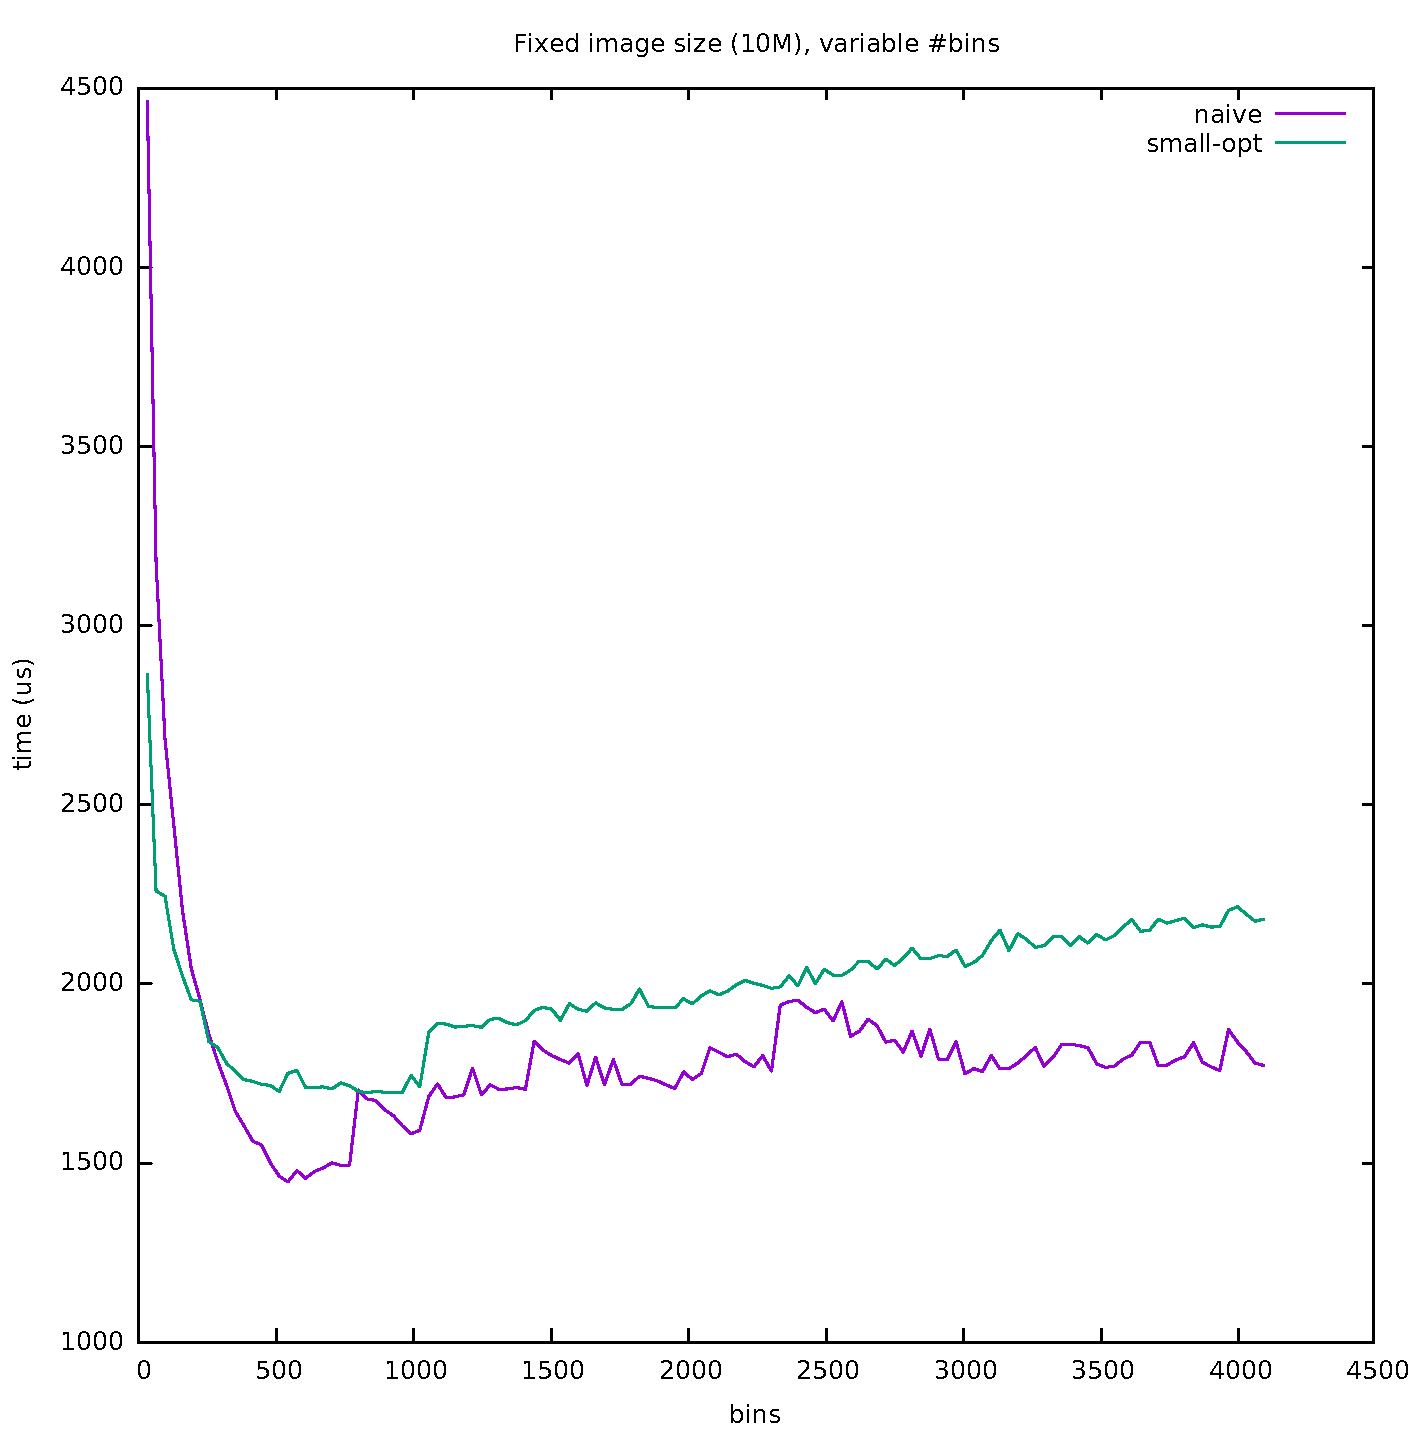
\includegraphics[width=0.6\linewidth]{img/graphs/10M-smallvarbins.pdf}
    \caption{10 million elements with a small variable bin count.}
    \label{fig:graph4}
\end{figure}

% should probably be rewritten in form which is better for reading flow,
% but I don't think Cosmin really cares - Joachim.
The histogram kernel optimised for small histogram sizes is around
20-30\% faster than the very simple naive version.
Both implementations see a spike around 1k bins.
This is probably the sign of some cache effects.
They are also very slow for very few bins.
This is because that we have a lot of synchronised writes to the same memory locations.


\section{Discussion}


%% \subsection{Atomic addition}
%% Using atomic addition yiels specific corner case issues, 
%% in the case for which we find a large number of datapoints falling into the same bin. 
%% In those cases atomic addition runs almost sequentially, 
%% therefore optimizations will not have had an effect.
%% This is however a very unlikely real world application scenario,
%% because of datasets are more likely to contain scattered datapoints.
%% Even though we find the histogram containing a small number of bins, 
%% we still see significant improvements compared to a naive implementation in figure \ref{fig:graph3} and \ref{fig:graph4}.

%% Imagine the unlikely case of a histogram of size 1. Even though it makes little sense,
%% the idea reveals a real bottleneck. Since all additions to the
%% histogram must be atomic, the reduction part of the algorithm for
%% such a small histogram
%% exposes exactly 0 parallelism! But as the size of the global histogram
%% expands, this problem becomes smaller and smaller.
%% Hence, we expect the parrallel implementation to perform better when the
%% histogram size expands, for a fixed input data size.
%% An example of this effect can be seen in \Cref{fig:graph4}.

\subsection{The Expense of Sorting}
Unfortunately, sorting data and keeping track of segments
introduces great deal of extra work. Currently, memory transfers are still the greater evil, but if we imagine a scenario where the kernels were working harder and streaming made more sense, sorting likely becomes the prime bottleneck. We have yet to see a way to get around this and at the same time fully utilize the shared memory on the GPU blocks. However, on a large input sorting is quicker than cache-ineffeciency (as shown in section \ref{section:bench} Benchmarks).

\subsection{Kernel fusion}
As seen in table~\Cref{table:nvprof0}, the relatively simple task of calculating the segment offsets
poses a significant overhead. This is because it requires a full pass over the \tt{inds} array.

The histogram kernel which is called right after the segment offset kernel also does a full
pass over the \tt{inds} in the exact same order. We then suggest that one way of reducing
this overhead is by doing the segment offset calculation in the histogram kernel while
writing the indices into the histogram.

We suspect that this will almost totally eliminate the overhead of calling the segment
offsets kernel, and thereby reducing the runtime with about 15-20\%.

\subsection{Streaming histogram computation}
The profiling also showed that a lot of time was spent on copying data to the device,
though we did not include those numbers in the benchmarks themselves. In a real
world scenario you would at some point need to copy a lot of data to the device.

For histograms larger than what fits in global device memory, we would like to split
the input array into smaller chunks, and work on them in turn.
This gives rise to the possibility of using streaming in order better utilize the hardware.
In this case we would like to overlap computation with copying.

CUDA streams gives us the possibility to do this in a fashion shown on figure~\ref{fig:cuda-stream}.
The figure shows copying to the device (HD),
histogram computation (K) and copying back the resulting histogram (DH).

\begin{figure}[htpb]
    \centering
    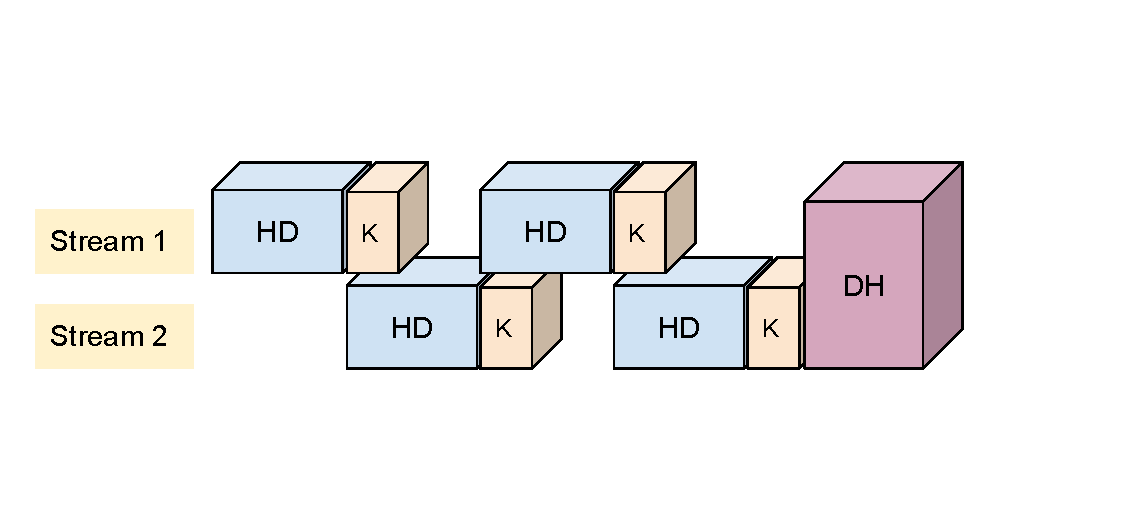
\includegraphics[width=0.8\linewidth]{img/cuda-stream.pdf}
    \captionof{table}{Using streams to overlap copying with computation.}
    \label{fig:cuda-stream}
\end{figure}

For this to work, we need to allocate buffers corresponding to 2 histogram computations.
Then while one buffer is filling up, we are calculating a histogram from the other
buffer. Both are commited to the same histogram.

Because memory copying vastly dominates the runtime of the implementation (90\%),
there is no need to use the optimsed histogram implementation, because the runtime
is limited by the fact that memory transfers are sequential.

We measure this by benchmarking with 1, 2 and 4 streams and on the CPU. 1 stream
is to check whether memory transfers are the dominating factor. This is because
using 1 stream makes sure that all the kernels are non-overlapping.

\begin{table}[htpb]
    \centering
    \begin{tabular}{l l}
        Method & Time \\
        \hline
        CPU & 9.64 s \\
        1 stream  & 4.91 s \\
        2 streams & 4.84 s \\
        4 streams & 4.92 s \\
        \hline
    \end{tabular}
    \caption{Time of streaming to the device}
    \label{tab:stream}
\end{table}

We test with a data size of 2G elements, and 400k bins. The result is shown in table~\ref{tab:stream}.
This is what we expected, because we deal with a lot of data, and memory transfers to the GPU is
relatively slow compared to computations.

\section{Conclusion}
It is in fact possible, to write a computationally efficient and scalable CUDA kernel,
to perform histogram computation for real world unsorted input data.
However the overhead from copying data,
causes the speedup from such an implementation to be much less significant than expected. Using streamning to hide memory latency only has an application if the computation time of kernels were larger (i.e. more work per thread is needed for efficiency).


% **************** The End ******************
\end{document}
